\documentclass{report}\usepackage[]{graphicx}\usepackage[]{color}
%% maxwidth is the original width if it is less than linewidth
%% otherwise use linewidth (to make sure the graphics do not exceed the margin)
\makeatletter
\def\maxwidth{ %
  \ifdim\Gin@nat@width>\linewidth
    \linewidth
  \else
    \Gin@nat@width
  \fi
}
\makeatother

\definecolor{fgcolor}{rgb}{0.345, 0.345, 0.345}
\newcommand{\hlnum}[1]{\textcolor[rgb]{0.686,0.059,0.569}{#1}}%
\newcommand{\hlstr}[1]{\textcolor[rgb]{0.192,0.494,0.8}{#1}}%
\newcommand{\hlcom}[1]{\textcolor[rgb]{0.678,0.584,0.686}{\textit{#1}}}%
\newcommand{\hlopt}[1]{\textcolor[rgb]{0,0,0}{#1}}%
\newcommand{\hlstd}[1]{\textcolor[rgb]{0.345,0.345,0.345}{#1}}%
\newcommand{\hlkwa}[1]{\textcolor[rgb]{0.161,0.373,0.58}{\textbf{#1}}}%
\newcommand{\hlkwb}[1]{\textcolor[rgb]{0.69,0.353,0.396}{#1}}%
\newcommand{\hlkwc}[1]{\textcolor[rgb]{0.333,0.667,0.333}{#1}}%
\newcommand{\hlkwd}[1]{\textcolor[rgb]{0.737,0.353,0.396}{\textbf{#1}}}%
\let\hlipl\hlkwb

\usepackage{framed}
\makeatletter
\newenvironment{kframe}{%
 \def\at@end@of@kframe{}%
 \ifinner\ifhmode%
  \def\at@end@of@kframe{\end{minipage}}%
  \begin{minipage}{\columnwidth}%
 \fi\fi%
 \def\FrameCommand##1{\hskip\@totalleftmargin \hskip-\fboxsep
 \colorbox{shadecolor}{##1}\hskip-\fboxsep
     % There is no \\@totalrightmargin, so:
     \hskip-\linewidth \hskip-\@totalleftmargin \hskip\columnwidth}%
 \MakeFramed {\advance\hsize-\width
   \@totalleftmargin\z@ \linewidth\hsize
   \@setminipage}}%
 {\par\unskip\endMakeFramed%
 \at@end@of@kframe}
\makeatother

\definecolor{shadecolor}{rgb}{.97, .97, .97}
\definecolor{messagecolor}{rgb}{0, 0, 0}
\definecolor{warningcolor}{rgb}{1, 0, 1}
\definecolor{errorcolor}{rgb}{1, 0, 0}
\newenvironment{knitrout}{}{} % an empty environment to be redefined in TeX

\usepackage{alltt}
\usepackage{amsmath, amssymb}
\usepackage{hyperref}
\usepackage{enumerate}
\IfFileExists{upquote.sty}{\usepackage{upquote}}{}
\begin{document}

\chapter{Multivariate Statistical Process Control with \texttt{mvMonitoring}}

This document serves to introduce engineers to the workflow necessary to follow in order to analyze multivariate process monitoring data via the \texttt{mvMonitoring} package.


%%%%%%%%%%%%%%%%%%%%%%%%%%%%%%%%%%%%%%%%%%%%%%%%%%%%%%%%%%%%%%%%%%%%%%%%%%%%%%%
%%%%%%  Introduction  %%%%%%%%%%%%%%%%%%%%%%%%%%%%%%%%%%%%%%%%%%%%%%%%%%%%%%%%%
%%%%%%%%%%%%%%%%%%%%%%%%%%%%%%%%%%%%%%%%%%%%%%%%%%%%%%%%%%%%%%%%%%%%%%%%%%%%%%%

\section{Introduction} \label{sec:intro}

This is the accompanying package to the research published by \cite{kazor_comparison_2016} and the previous chapter. The \texttt{mvMonitoring} package is designed to make simulation of multi-state multivariate process monitoring statistics easy and straightforward, as well as streamlining the statistical process monitoring component. This package can be downloaded from GitHub by running the following:
\begin{knitrout}
\definecolor{shadecolor}{rgb}{0.969, 0.969, 0.969}\color{fgcolor}\begin{kframe}
\begin{alltt}
 \hlstd{devtools}\hlopt{::}\hlkwd{install_github}\hlstd{(}\hlstr{"gabrielodom/mvMonitoring"}\hlstd{,} \hlkwc{auth_token} \hlstd{=} \hlstr{"tokenHere"}\hlstd{)}
\end{alltt}
\end{kframe}
\end{knitrout}
\noindent where you create the value of ``tokenHere'' by generating a personal access token (PAT) at \url{https://github.com/settings/tokens} and copying the quoted string to this argument.


We outline this vignette as follows. In Section \ref{sec:D_Motivation}, we discuss the motivation for creating this package, and briefly explain the utility of multi-state process monitoring. In Section \ref{sec:D_DataGen}, we offer a thorough explination of how to generate the synthetic data we employed to test and compare the new multi-state modification of the process monitoring setup with the \texttt{mspProcessData} function. In Section \ref{sec:D_Train}, we describe the necessary information and data formatting to effectively train the fault detection algorithm using the \texttt{mspTrain} function. Then, in Section \ref{sec:D_Alarms}, we list and explain the necessary inputs to the \texttt{mspMonitor} and \texttt{mspWarning} functions and examine their outputs. Section \ref{sec:D_Workflow} shows a step-by-step walkthrough of how to implement the four \texttt{mvMonitoring} functions in practice. We offer some concluding remarks in Section \ref{sec:D_Conclusion}.



%%%%%%%%%%%%%%%%%%%%%%%%%%%%%%%%%%%%%%%%%%%%%%%%%%%%%%%%%%%%%%%%%%%%%%%%%%%%%%%
%%%%%%  Motivation  %%%%%%%%%%%%%%%%%%%%%%%%%%%%%%%%%%%%%%%%%%%%%%%%%%%%%%%%%%%
%%%%%%%%%%%%%%%%%%%%%%%%%%%%%%%%%%%%%%%%%%%%%%%%%%%%%%%%%%%%%%%%%%%%%%%%%%%%%%%

\section{Motivation} \label{sec:D_Motivation}

\subsection{Why use \texttt{mvMonitoring}?}
The \texttt{mvMonitoring} package can be used to detect outliers in a correlated, non-Gaussian multivariate process with non-linear, non-stationary, or autocorrelated feature behavior. These process outliers are often indicative of system fault. The naive (but unfortunately common) approach to multivariate process monitoring is to use expert opinion to identify a few important features to monitor visually, and raise an alarm if these features travel outside pre-defined normal operating boundaries.

However, this split univariate approach fails to account for the correlated nature of the process features, so some engineers have taken to monitoring the system as a single correlated multivariate process rather than a collection of independent univariate processes. In the literature review of the motivating papers, the authors cite how this approach has benefited the science of process monitoring as a whole. Unfortunately, this approach has its own shortcomings. One such complication is that monitoring a multivariate process in its original feature space can lead to exorbitant computational costs. Additionally, correlated multivariate process over many features may be noisy and often retain redundant information. To combat these issues, \emph{principal components analysis} (PCA) and its many modifications have been employed to assist in monitoring multivariate processes as a whole. This package is an implementation of one such PCA modification.


\subsection{Multi- or Single-State AD-PCA}
\emph{Adaptive-Dynamic} PCA (AD-PCA), thoroughly discussed in \cite{kazor_comparison_2016} as well as in the previous chapter, accounts for non-linearity, non-stationarity, and autocorrelation in non-Gaussian multivariate processes. As an additional layer of complexity within this model, consider such a process with multiple known system states. \emph{Multi-State} monitoring is thus a modification to PCA which accounts for multiple process states and models them separately. States can be any mutually exclusive blocking factor, and states do not necessarily follow a strict order. Then, Multi-State AD-PCA (MSAD-PCA) allows process engineers to account for distinct process states. Specifically, this modification should be used when features under different process states have different means, correlations, variances, or some combination of these three.



%%%%%%%%%%%%%%%%%%%%%%%%%%%%%%%%%%%%%%%%%%%%%%%%%%%%%%%%%%%%%%%%%%%%%%%%%%%%%%%
%%%%%%  mspProcessData  %%%%%%%%%%%%%%%%%%%%%%%%%%%%%%%%%%%%%%%%%%%%%%%%%%%%%%%
%%%%%%%%%%%%%%%%%%%%%%%%%%%%%%%%%%%%%%%%%%%%%%%%%%%%%%%%%%%%%%%%%%%%%%%%%%%%%%%

\section{Simulating Data with \texttt{mspProcessData}} \label{sec:D_DataGen}
The \texttt{mspProcessData} function generates three-dimensional multi-state or single-state non-linear, non-stationary, and autocorrelated process observations. We follow the seminal work of \cite{dong_batch_1996} for generation of the foundational stationary and independent features.


\subsection{Latent Feature Creation}
So that the simulated features have non-zero correlations, Dong and McAvoy created their three features all as polynomial functions of a single latent variable $t_s$, where $s = 1, \ldots, \omega$ is the observational index of the process.

\subsubsection{Autocorrelated and Non-Stationary Error}
The \texttt{mspProcesData} function induces autocorrelation in $t$ through its errors, $\varepsilon_s$, where
\[
  \varepsilon_1 \sim \mathcal{N}\left(\frac{1}{2}(a + b)(1 - \varphi), \frac{b - a}{12} (1 - \varphi ^ 2)\right),
\]
where $a = 0.01$ and $b = 2$. Now, we define the first-order autoregressive process on $\varepsilon_s$ by
\[
  \varepsilon_s = \varphi\varepsilon_{s - 1} + (1 - \varphi)\varepsilon,
\]
where $\varepsilon$ is a random innovation drawn from the Normal distribution defined in the previous expression, and the autocorrelation component $\varphi = 0.75$. The mean and variance multipliers are the mean and variance of a random variable from the $\text{uniform}_{[a,b]}$ distribution.

\subsubsection{The Non-Linear Latent Process}
This $t$ vector will be sinusoidal with period $\omega = 7 * 24 * 60$ (signifying a weekly period in  minute-level observations). We then synthesize a $t$ by taking
\[
  t^*_s = -\cos\left( \frac{2\pi}{\omega} s \right) + \epsilon_s,
\]
and then scaling $t^*$ to
\[
  t = \frac{(b - a)(t^*_s - \text{min}(t^*_s))}{\text{max}(t^*_s) - \text{min}(t^*_s)} + a.
\]
Finally then, the $t$ vector will lie entirely in $[a,b]$.


\subsection{Single-State and Multi-State Features}

\subsubsection{Single State Features}
First \texttt{mspProcessData} simulates three features, with each feature operating under $k$ different states. Let $\langle x_k(t_s), y_k(t_s), z_k(t_s) \rangle$ be the process evaluated at $t_s$ within State $k$. These are the three features under State 1 (in control, or \emph{IC}) as three functions of $t$:
\begin{align}
x(\textbf{t}) &\equiv \textbf{t} + \boldsymbol\varepsilon_1, \\
y(\textbf{t}) &\equiv \textbf{t} ^ 2 - 3 * \textbf{t} + \boldsymbol\varepsilon_2, \\
z(\textbf{t}) &\equiv -\textbf{t} ^ 3 + 3 * \textbf{t} ^ 2 + \boldsymbol\varepsilon_3,
\end{align}
where $\varepsilon_i \sim N(0, 0.01),\ 1 = 1, 2, 3$. The \texttt{mspProcessData} function calls the internal \texttt{processNOCdata} function to generate IC single-state observations.

\subsubsection{Multi-State Features}
The multi-state feature expression is induced by rotation and scaling of certain sets of observations. To induce a three-state, hourly switching process (the default), the \texttt{mspProcessData} function will create a label column that switches from ``1'' to ``2'' to ``3'' every hour. State ``1'' will be the features generated under the single-state assumption, while State ``2'' and State ``3'' are generated as follows. These states will be scaled rotations of the current $\langle x,y,z \rangle$ set. The second state is yaw, pitch, and roll rotated by (0, 90, 30) degrees, and the scales are multiplied by (1, 0.5, 2). The third state is yaw, pitch, and roll rotated by (90, 0, -30) degrees, and the scales are multiplied by (0.25, 0.1, 0.75). That is,
\begin{enumerate}
\item $\mathcal{S}_1$: $\textbf{X}(t_s) := \langle x(t_s), y(t_s), z(t_s)\rangle$.

\item $\mathcal{S}_2$: $\textbf{X}(t_s) := \langle x(t_s), y(t_s), z(t_s)\rangle \cdot \textbf{P}_1\boldsymbol\Lambda_1$, where
\[
  \textbf{P}_1 = \begin{bmatrix}
  0    &  0.50 & -0.87 \\
  0    &  0.87 &  0.50 \\
  1    &  0    &  0
  \end{bmatrix}
\]
is the orthogonal rotation matrix for a yaw, pitch and roll degree change of $\langle 0^{\circ}, 90^{\circ}, 30^{\circ} \rangle$, and $\boldsymbol\Lambda_1 = \text{diag}(1, 0.5, 2)$ is a diagonal scaling matrix.

\item $\mathcal{S}_3$: $\textbf{X}(t_s) := \langle x(t_s), y(t_s), z(t_s)\rangle \cdot \textbf{P}_2\boldsymbol\Lambda_2$, where
\[
  \textbf{P}_2 = \begin{bmatrix}
  0    &  0.87 & -0.50 \\
  -1    &  0    &  0    \\
  0    &  0.50 &  0.87
  \end{bmatrix}
\]
is the orthogonal rotation matrix for a yaw, pitch and roll degree change of $\langle 90^{\circ}, 0^{\circ}, -30^{\circ} \rangle$, and $\boldsymbol\Lambda_2 = \text{diag}(0.25, 0.1, 0.75)$ is a diagonal scaling matrix.
\end{enumerate}

These rotation matrices $\textbf{P}_1$ and $\textbf{P}_2$ turn the states in three-dimensional space so that the states are at right angles to each other in at least one dimension, and the scaling matrices $\boldsymbol\Lambda_1$ and $\boldsymbol\Lambda_2$ inflate or deflate the process variances along each principal component. The \texttt{mspProcessData} function calls the internal function \texttt{dataStateSwitch} which splits the observations by state and applies the state-specific rotation and scaling through the internal \texttt{rotateScale3D} function.


\subsection{Synthetic Fault Induction}
Faults can be introduced to single- or multi-state data via the \texttt{mspProcessData} function. The default fault start index is 8500, or roughly 84\% through the cycle of 10,080 observations. These faults are added through the internal \texttt{faultSwitch} function.
\begin{enumerate}
\item Fault 1A is a positive shift to all three features before state rotation: $\textbf{X}^*(t_s) = \textbf{X}(t_s) + 2,\ s \ge 8500$.
%
\item Fault 1B is a positive shift to the $x$ feature before state rotation: $x^*(t_s) = x(t_s) + 2,\ s \ge 8500$.
%
\item Fault 1C is a positive shift to the $x$ and $z$ features in State 3 only and \emph{after} state rotation: $x^*(t_s) = x(t_s) + 2,\ z^*(t_s) = z(t_s) + 2,\ s \ge 8500$.
%
\item Fault 2A is a positive drift across all the process monitoring features before state rotation: $\textbf{X}^*(t_s) = \textbf{X}(t_s) + (s - 8500)\times 10^{-3}$, $s > 8500$.
%
\item Fault 2B is a positive drift across the $y$ and $z$ process monitoring features before state rotation: $y^*(t_s) = y(t_s) + (s - 8500)\times 10^{-3},\ z^*(t_s) = z(t_s) + (s - 8500)\times 10^{-3}$, $s > 8500$.
%
\item Fault 2C is a negative drift in the $y$ process monitoring feature in State 2 only and \emph{after} state rotation: $y^*(t_s) = y(t_s) - 1.5 \times \frac{s - 8500}{10080 - 8500}$, for $s > 8500$.
%
\item Fault 3A is an amplification of the underlying latent variable $t$ for all features. The maximum latent drift of this fault will be 5 + 1: $\textbf{X}^*(t_s) = \textbf{X}(t_s^*),\ s > 8500$, where $t_s^* = \left[\frac{5(s - 8500)}{\omega - 8500} + 1\right]t_s$.
%
\item Fault 3B is a mutation of the underlying latent variable $t$ for the $z$ feature: $z^*(t_s) = z(\log t_s^*)$, $s \ge 8500$. This fault will dampen the underlying latent effect for $z$ if $t_s > 1$ and amplify this effect if $t_s < 1$.
%
\item Fault 3C is a polynomial mutation of the error for the $y$ feature in State 2 only and \emph{after} state rotation: $y^*(t_s) = y(t_s) + 2 * \textbf{e}_3(s) - 0.25$, for $s > 8500$.
\end{enumerate}


\subsection{Putting it all together\ldots}
The \texttt{mspProcessData} function can generate weeks' worth of non-linear, non-stationary, autocorrelated, multi-state, multivariate process data useful to test new process monitoring techniques. Users can generate IC observations to measure false alarm rates, or induce one of nine pre-built faults to test detection time and consistency with repeated Monte Carlo sampling. We expect this function will generate interesting data useful enough to compare new and improved process monitoring techniques with existing methods. A detailed description of this function's inputs and outputs are shown in Section \ref{sec:D_Workflow}.



%%%%%%%%%%%%%%%%%%%%%%%%%%%%%%%%%%%%%%%%%%%%%%%%%%%%%%%%%%%%%%%%%%%%%%%%%%%%%%%
%%%%%%  mspTrain  %%%%%%%%%%%%%%%%%%%%%%%%%%%%%%%%%%%%%%%%%%%%%%%%%%%%%%%%%%%%%
%%%%%%%%%%%%%%%%%%%%%%%%%%%%%%%%%%%%%%%%%%%%%%%%%%%%%%%%%%%%%%%%%%%%%%%%%%%%%%%

\section{Training with \texttt{mspTrain}} \label{sec:D_Train}

The \texttt{mspTrain} function will generate projection matrices and test statistic thresholds from training data matrices. It requires data matrices to be in the \texttt{xts} matrix format.


\subsection{The \texttt{xts} Data Matrix}
An \texttt{xts} data matrix is first and foremost a matrix, \emph{not} a data frame. For users very familiar with data frame manipulation (with \texttt{dplyr} for instance), the slight but profound differences between manipulating matrices and data frames quickly become apparent. Because of the class requirements for matrices, \emph{all} features must be integer or double vectors. The \texttt{mspTrain} function cannot train on non-numeric information.

The \texttt{xts} object class stands for \emph{extendible time series} and comes from the package \texttt{xts}, which is built on the package \texttt{zoo}. The date and time information for the multivariate stochastic process (necessarily as \texttt{POSIX} objects) are stored as the row indices of \texttt{xts} matrices. We recommend the package \texttt{lubridate} for manipulating \texttt{POSIX} objects.


\subsection{The State Vector}
The state membership (or \emph{class}) vector of the data matrix is the column of integer values corresponding to the generation state of the observation. When implementing single-state AD-PCA, this class vector will simply be a numeric column of the same value -- for instance, 1. However, for MSAD-PCA, the class vector indicates from which state each observation has been drawn.

The \texttt{mspTrain} function will split the observations by the class vector, apply single-state AD-PCA to each class, then return the class-specific projection matrices and thresholds. Because of this split-apply-combine strategy, users must ensure that one or more classes are not too ``rare'' -- that is, the class sample sizes should be sufficiently large to allow for stable covariance matrix inversion. For $p$ features (including lags), stable covariance inversion requires a class sample size near $p ^ 2 / 2$ at minimum. Because of this, attention must be given to model parsimony -- we recommend against blocking observations on a factor unless that factor has sufficent observations and significantly affects the observations' mean vector or covariance matrix.


\subsection{Adaptive and Dynamic Modeling}
Because of the non-linear, non-stationary, and autocorrelated nature of some process monitoring applications, the \texttt{mspTrain} function allows users to include lags of all feature variables. Including lags of the features in the data matrix (dynamic) can significantly reduce the negative effects of modeling autocorrelated observations. Further, the \texttt{mspTrain} function includes the option to update the training window over time. Re-estimating the projection matrix and test statistic thresholds at pre-specified time intervals  (adaptive) can reduce the negative effects of non-linearity and non-stationarity when modeling the observations. The idea is to divide a non-linear and non-stationary process between some equally-spaced boundaries (every day, for instance), so that the process becomes locally linear and stationary within these boundaries. As time progresses, the oldest observations are ``forgotten'' and the newest observations are ``learned''. This causes the projection and IC thresholds to ``adapt'' over time.


\subsection{Model Training}
After the observations have been split by class, the \texttt{mspTrain} function will call the internal function \texttt{processMonitor}, which subsequently calls the internal function \texttt{faultFilter}. This function will calculate a linear projection matrix of the data by taking the PCA of the training data matrix. The observations will then be projected linearly into a reduced-feature subspace which preserves a chosen proportion of the energy of the training data, where the energy of a matrix is the relative sum of eigenvalues of that matrix. The default proportion is 90\%. This projection is calculated by the internal \texttt{pca} function.

Furthermore, non-parametric threshold values are calculated for the two process monitoring statistics -- \emph{Squared Prediction Error} (SPE) and \emph{Hotelling's} $T^2$ ($T^2$). These monitoring statistics are described in the motivating paper (Chapter \ref{chap:MS_MVSPC}). These threshold values are calculated by the internal \texttt{threshold} function, and passed up through the function pipe to be returned by \texttt{mspTrain}. The $\alpha$-level of the nonparametric threshold is controlled by the user, but defaults to 0.001.

Finally, the \texttt{mspTrain} function will remove any observation(s) which would cause an alarm from the training data set. The alarm-free observations will be returned in one \texttt{xts} matrix, while the alarmed observations will be returned by another. The alarm criteria are discussed in Section \ref{sec:D_Alarms}. When training the process monitor, pay attention to any observations flagged as alarms. The proportion of observations flagged as faults may be higher than the $\alpha$-level specified, so some tuning may be necessary. As with the \texttt{mspProcessData} function, a detailed description of the inputs and outputs from the \texttt{mspTrain} function are shown in Section \ref{sec:D_Workflow}.



%%%%%%%%%%%%%%%%%%%%%%%%%%%%%%%%%%%%%%%%%%%%%%%%%%%%%%%%%%%%%%%%%%%%%%%%%%%%%%%
%%%%%%  mspMonitor and mspWarning  %%%%%%%%%%%%%%%%%%%%%%%%%%%%%%%%%%%%%%%%%%%%
%%%%%%%%%%%%%%%%%%%%%%%%%%%%%%%%%%%%%%%%%%%%%%%%%%%%%%%%%%%%%%%%%%%%%%%%%%%%%%%

\section{Monitor and Issue Alarms with \texttt{mspMonitor} and \texttt{mspWarning}} \label{sec:D_Alarms}

After training the model with \texttt{mspTrain}, the projection matrices and non-parametric monitoring statistic thresholds can be used to flag incoming observations which are potentially out of control. The \texttt{mspMonitor} function was instead designed to test a single incoming observation at a time via a script or batch file, but \emph{can} check every observation in a test matrix, which is useful for analyzing past data. To this end, the \texttt{mspMonitor} function projects a single observation with the class projection matrices returned by \texttt{mspTrain} and checks the observation's \emph{SPE} and $T^2$ statistics against the thresholds also returned by \texttt{mspTrain}. The \texttt{mspMonitor} function will then append the monitoring statistic values and indicators to the end of the observation row. Indicator values will be returned as a ``1'' if the values of these statistics exceed their IC thresholds. This new appended observation will be passed to the \texttt{mspWarning} function.

The \texttt{mspWarning} function takes in an observation returned by the \texttt{mspMonitor} function and an integer value (denoted $r$ for this discussion) dictating the number of sequential flagged observations observed before an alarm is raised. If an observation returned by the \texttt{mspMonitor} function has positive statistic indicator values for either the SPE or $T^2$ monitoring statistics, then the \texttt{mspWarning} function will query the most recent $r$ observations for other flags. If all $r$ observations are positive for anomalies, then the \texttt{mspWarning} function will issue an alarm. The number of flags necessary to trigger an alarm defaults to 5. However, this default value depends heavily on the scale of the data: for continuous observations aggregated and recorded every five seconds, the number of sequential flags necessary to trigger an alarm could be much higher, perhaps even 20 or more. In contrast, for observations aggregated to the 10-minute-scale, only three sequential flags may be necessary.

In future updates of this package, this function will also have an option to issue an alarm if a critical mass of non-sequential flags is reached in a set period of observations. This modification may be necessary if the observation level becomes more fine than the 1-minute-level. Additionally, this function will also be equipped to take in a cell phone number and service provider and issue an alarm via SMS through email. Detailed descriptions of the inputs and outputs from the \texttt{mspMonitor} and \texttt{mspWarning} functions are shown in the next section.



%%%%%%%%%%%%%%%%%%%%%%%%%%%%%%%%%%%%%%%%%%%%%%%%%%%%%%%%%%%%%%%%%%%%%%%%%%%%%%%
%%%%%%  Example Workflow  %%%%%%%%%%%%%%%%%%%%%%%%%%%%%%%%%%%%%%%%%%%%%%%%%%%%%
%%%%%%%%%%%%%%%%%%%%%%%%%%%%%%%%%%%%%%%%%%%%%%%%%%%%%%%%%%%%%%%%%%%%%%%%%%%%%%%

\section{Example Simulation Workflow} \label{sec:D_Workflow}

This section provides a fully commented code walk-through for the main \texttt{msp*} functions in the \texttt{mvMonitoring} package. This package depends on a few other packages, but most of these dependencies are on commonly-used packages. The exception is \texttt{BMS}.
\begin{knitrout}
\definecolor{shadecolor}{rgb}{0.969, 0.969, 0.969}\color{fgcolor}\begin{kframe}
\begin{alltt}
\hlkwd{library}\hlstd{(devtools)}
\hlkwd{library}\hlstd{(xts)}
\hlcom{# install.packages("BMS") # If necessary}
\hlkwd{build}\hlstd{(}\hlstr{"C:/Users/gabriel_odom/Documents/GitHub/mvMonitoring/mvMonitoring"}\hlstd{)}
\end{alltt}
\begin{verbatim}
## [1] "C:/Users/gabriel_odom/Documents/GitHub/mvMonitoring/mvMonitoring_0.1.1.tar.gz"
\end{verbatim}
\begin{alltt}
\hlkwd{library}\hlstd{(mvMonitoring)}
\end{alltt}
\end{kframe}
\end{knitrout}


\subsection{Generating Synthetic Data}
First begin by generating multi-state data from a fault scenario. This code will yield observations under Fault 2A, as described the Synthetic Fault Induction section. We choose the default options for the period length (7 days * 24 hours * 60 minutes = 10,080 observations), the starting index of the fault (8500 out of 10080), and the time stamp for beginning the data is 16 May of 2016 at 10:00AM (my wedding anniversary). As we can see from the \texttt{str()} function, we have an \texttt{xts} matrix with 10080 rows and four columns (the state indicator and the three features).

\begin{knitrout}
\definecolor{shadecolor}{rgb}{0.969, 0.969, 0.969}\color{fgcolor}\begin{kframe}
\begin{alltt}
\hlstd{fault1A_xts} \hlkwb{<-} \hlkwd{mspProcessData}\hlstd{(}\hlkwc{faults} \hlstd{=} \hlstr{"A1"}\hlstd{,}
                              \hlkwc{period} \hlstd{=} \hlnum{7} \hlopt{*} \hlnum{24} \hlopt{*} \hlnum{60}\hlstd{,}
                              \hlkwc{faultStartIndex} \hlstd{=} \hlnum{8500}\hlstd{,}
                              \hlkwc{startTime} \hlstd{=} \hlstr{"2015-05-16 10:00:00 CST"}\hlstd{)}
\hlkwd{str}\hlstd{(fault1A_xts)}
\end{alltt}
\begin{verbatim}
## An 'xts' object on 2015-05-16 10:00:00/2015-05-23 09:59:00 containing:
##   Data: num [1:10080, 1:4] 1 1 1 1 1 1 1 1 1 1 ...
##  - attr(*, "dimnames")=List of 2
##   ..$ : NULL
##   ..$ : chr [1:4] "state" "x" "y" "z"
##   Indexed by objects of class: [POSIXct,POSIXt] TZ: 
##   xts Attributes:  
##  NULL
\end{verbatim}
\end{kframe}
\end{knitrout}


\subsection{Train the Fault Detection Threshold}
Now that these observations are generated and stored in memory, the \texttt{mspTrain} function can train the MSAD-PCA model. The last 1620 observations (27 hours' worth) will be saved for testing. The \texttt{mspTrain} function takes in the training data set partitioned between the observation and the label column. If this function errors, make sure the label column is not included in the data matrix -- this will cause a singularity in the data. The function will
\begin{enumerate}
\item Train on the first three days' worth of observations, as set by \texttt{trainObs}.
%
\item Scan the fourth day for anomalies, as set by \texttt{updateFreq}.
%
\item Remove any alarmed observations.
%
\item ``Forget'' the first day's observations.
%
\item ``Learn'' the non-alarmed observations from the fourth day.
%
\item Retrain and repeat until the end of the data matrix
\end{enumerate}


Furthermore, the \texttt{Dynamic = TRUE} option means that the \texttt{mspTrain} function will include the lags specified by the \texttt{lagsIncluded} argument. Finally, the number of sequential anomalous observations necessary to raise an alarm is set at 5 by the \texttt{faultsToTriggerAlarm} argument. These last three arguments are set to their defaults.
\begin{knitrout}
\definecolor{shadecolor}{rgb}{0.969, 0.969, 0.969}\color{fgcolor}\begin{kframe}
\begin{alltt}
\hlstd{train1A_xts} \hlkwb{<-} \hlstd{fault1A_xts[}\hlnum{1}\hlopt{:}\hlnum{8461}\hlstd{,]}
\hlcom{# This function will run in 13 seconds on the author's machine.}
\hlstd{train1A_ls} \hlkwb{<-} \hlkwd{mspTrain}\hlstd{(}\hlkwc{data} \hlstd{= train1A_xts[,}\hlopt{-}\hlnum{1}\hlstd{],}
                       \hlkwc{labelVector} \hlstd{= train1A_xts[,}\hlnum{1}\hlstd{],}
                       \hlkwc{trainObs} \hlstd{=} \hlnum{3} \hlopt{*} \hlnum{24} \hlopt{*} \hlnum{60}\hlstd{,}
                       \hlkwc{updateFreq} \hlstd{=} \hlnum{1} \hlopt{*} \hlnum{24} \hlopt{*} \hlnum{60}\hlstd{,}
                       \hlkwc{Dynamic} \hlstd{=} \hlnum{TRUE}\hlstd{,}
                       \hlkwc{lagsIncluded} \hlstd{=} \hlnum{0}\hlopt{:}\hlnum{1}\hlstd{,}
                       \hlkwc{faultsToTriggerAlarm} \hlstd{=} \hlnum{5}\hlstd{)}
\hlkwd{str}\hlstd{(train1A_ls)}
\end{alltt}
\begin{verbatim}
## List of 4
##  $ FaultChecks    :An 'xts' object on 2015-05-19 08:59:00/2015-05-22 07:00:00 containing:
##   Data: num [1:4142, 1:5] 0.28 0.201 1.208 0.919 0.418 ...
##  - attr(*, "dimnames")=List of 2
##   ..$ : NULL
##   ..$ : chr [1:5] "SPE" "SPE_Flag" "T2" "T2_Flag" ...
##   Indexed by objects of class: [POSIXct,POSIXt] TZ: 
##   xts Attributes:  
##  NULL
##  $ Non_Alarmed_Obs:An 'xts' object on 2015-05-19 08:59:00/2015-05-22 07:00:00 containing:
##   Data: num [1:4142, 1:7] 2 3 1 1 1 1 1 1 1 1 ...
##  - attr(*, "dimnames")=List of 2
##   ..$ : NULL
##   ..$ : chr [1:7] "state" "x" "y" "z" ...
##   Indexed by objects of class: [POSIXct,POSIXt] TZ: 
##   xts Attributes:  
##  NULL
##  $ Alarms         :An 'xts' object of zero-width
##  $ TrainingSpecs  :List of 3
##   ..$ 1:List of 6
##   .. ..$ SPE_threshold   : Named num 4.29
##   .. .. ..- attr(*, "names")= chr "99.9%"
##   .. ..$ T2_threshold    : Named num 62.6
##   .. .. ..- attr(*, "names")= chr "99.9%"
##   .. ..$ projectionMatrix: num [1:6, 1:2] 0.422 -0.386 0.435 0.431 -0.318 ...
##   .. ..$ LambdaInv       : num [1:2, 1:2] 0.204 0 0 1.606
##   .. ..$ muTrain         : Named num [1:6] 1.37 -2.1 2.95 1.36 -2.06 ...
##   .. .. ..- attr(*, "names")= chr [1:6] "x" "y" "z" "x.1" ...
##   .. ..$ RootPrecisTrain : num [1:6, 1:6] 2.64 0 0 0 0 ...
##   .. ..- attr(*, "class")= chr [1:2] "threshold" "pca"
##   ..$ 2:List of 6
##   .. ..$ SPE_threshold   : Named num 1.16
##   .. .. ..- attr(*, "names")= chr "99.9%"
##   .. ..$ T2_threshold    : Named num 74.2
##   .. .. ..- attr(*, "names")= chr "99.9%"
##   .. ..$ projectionMatrix: num [1:6, 1:3] -0.4957 -0.0668 0.4887 -0.5236 -0.1866 ...
##   .. ..$ LambdaInv       : num [1:3, 1:3] 0.284 0 0 0 0.712 ...
##   .. ..$ muTrain         : Named num [1:6] 2.978 -0.566 -4.508 2.95 -0.592 ...
##   .. .. ..- attr(*, "names")= chr [1:6] "x" "y" "z" "x.1" ...
##   .. ..$ RootPrecisTrain : num [1:6, 1:6] 1.08 0 0 0 0 ...
##   .. ..- attr(*, "class")= chr [1:2] "threshold" "pca"
##   ..$ 3:List of 6
##   .. ..$ SPE_threshold   : Named num 8.04
##   .. .. ..- attr(*, "names")= chr "99.9%"
##   .. ..$ T2_threshold    : Named num 80.8
##   .. .. ..- attr(*, "names")= chr "99.9%"
##   .. ..$ projectionMatrix: num [1:6, 1:2] -0.392 -0.452 -0.454 0.163 -0.462 ...
##   .. ..$ LambdaInv       : num [1:2, 1:2] 0.278 0 0 0.493
##   .. ..$ muTrain         : Named num [1:6] 0.528 0.268 1.413 0.57 0.254 ...
##   .. .. ..- attr(*, "names")= chr [1:6] "x" "y" "z" "x.1" ...
##   .. ..$ RootPrecisTrain : num [1:6, 1:6] 17.4 0 0 0 0 ...
##   .. ..- attr(*, "class")= chr [1:2] "threshold" "pca"
\end{verbatim}
\end{kframe}
\end{knitrout}
The \texttt{mspTrain} function returns a list of four objects:
\begin{enumerate}
\item \texttt{FaultChecks}: An \texttt{xts} matrix of monitoring statistics and associated indicators for all observations after the burn-in of \texttt{trainObs}. It will have 10080 - \texttt{trainObs} number of rows and five columns:
	\begin{enumerate}
	\item \texttt{SPE}: the SPE statistic for each observation.
    %
    \item \texttt{SPE\_Flag}: an indicator showing if the SPE statistic for that observation is beyond the calculated threshold; 0 is normal, 1 is flagged.
    %
    \item \texttt{T2}: the $T^2$ statistic for each observation.
    %
    \item \texttt{T2\_Flag}: an indicator showing if the $T^2$ statistic for that observation is beyond the calculated threshold; 0 is normal, 1 is flagged.
    %
    \item \texttt{Alarm}: an indicator showing if the observation is in a sequence of flagged observations; 0 is normal, 1 is alarmed.
	\end{enumerate}
%
\item \texttt{Non\_Alarmed\_Obs}: An \texttt{xts} matrix will all observations with an alarm code of 0 from \texttt{FaultChecks}. Of note, this matrix contains the data, while the \texttt{FaultChecks} matrix only contains the monitoring statistics and indicators.
%
\item \texttt{Alarms}: An \texttt{xts} matrix of all the observations removed from the training data matrix.
%
\item \texttt{TrainingSpecs}: a list with length equal to the number of classes -- in this case 3. For each class, this list contains a list of six objects:
	\begin{enumerate}
	\item \texttt{SPE\_Threshold}: a named numeric scalar of the $1 - \alpha$ percentile of the non-parametric estimate of the SPE statistic density.
    %
    \item \texttt{T2\_Threshold}: a named numeric scalar of the $1 - \alpha$ percentile of the non-parametric estimate of the $T^2$ statistic density.
    %
    \item \texttt{projectionMatrix}: The $p \times q$ matrix of eigenvectors necessary to project a $p$-dimensional observation to $q$ dimensions. This is necessary to reduce the dimension of any test observation, and is used in calculating the SPE statistic for test observations.
    %
    \item \texttt{LambdaInv}: The inverse of the diagonal $q \times q$ matrix of eigenvalues. This matrix is used to calculate the $T^2$ statistic for test observations.
    %
    \item \texttt{muTrain}: The mean vector of the training observations. This is used to center the test observations on the training mean.
    %
    \item \texttt{RootPrecisTrain}: The $p \times p$ diagonal matrix of the inverse square roots of the feature variances. This is used to scale the test observations into the training scale.
	\end{enumerate}
\end{enumerate}


\subsection{Test New Observations for Anomalies}
The training data summary was given by \texttt{mspTrain}, so this information can now be used to monitor incoming observations for system faults.

\subsubsection{Adding Lagged Features}
First, concatenate the last given observation from the training set as ``row 0'' of the test data set. This will enable \texttt{mspMonitor} to include lag-1 features. Similarly, one would include the last $k$ observations of the training set should the process dictate the need for any lag-$k$ features. Because the Fault Start Index was set to 8500, this testing window will show the change point between observations generated under normal conditions and those generated under a fault state.
\begin{knitrout}
\definecolor{shadecolor}{rgb}{0.969, 0.969, 0.969}\color{fgcolor}\begin{kframe}
\begin{alltt}
\hlstd{test1A_xts} \hlkwb{<-} \hlstd{fault1A_xts[}\hlnum{8460}\hlopt{:}\hlnum{8520}\hlstd{,} \hlopt{-}\hlnum{1}\hlstd{]}
\hlstd{lagTest1A_xts} \hlkwb{<-} \hlkwd{lag.xts}\hlstd{(test1A_xts,} \hlnum{0}\hlopt{:}\hlnum{1}\hlstd{)}
\hlstd{lagTest1A_xts} \hlkwb{<-} \hlkwd{cbind}\hlstd{(fault1A_xts[}\hlnum{8461}\hlopt{:}\hlnum{8520}\hlstd{,}\hlnum{1}\hlstd{],}
                       \hlstd{lagTest1A_xts[}\hlopt{-}\hlnum{1}\hlstd{,])}
\hlkwd{head}\hlstd{(lagTest1A_xts)}
\end{alltt}
\begin{verbatim}
##                     state         x         y         z       x.1
## 2015-05-22 07:00:00     1 0.5454353 -1.494528 0.9296569 0.4159290
## 2015-05-22 07:01:00     1 0.5752773 -1.638525 1.1806822 0.5454353
## 2015-05-22 07:02:00     1 0.5381703 -1.448424 1.0029127 0.5752773
## 2015-05-22 07:03:00     1 0.6097887 -1.320156 0.9345597 0.5381703
## 2015-05-22 07:04:00     1 0.8534018 -1.555631 1.0922745 0.6097887
## 2015-05-22 07:05:00     1 0.7252695 -1.792569 1.1605990 0.8534018
##                            y.1       z.1
## 2015-05-22 07:00:00  0.1063122 0.3767823
## 2015-05-22 07:01:00 -1.4945284 0.9296569
## 2015-05-22 07:02:00 -1.6385255 1.1806822
## 2015-05-22 07:03:00 -1.4484243 1.0029127
## 2015-05-22 07:04:00 -1.3201558 0.9345597
## 2015-05-22 07:05:00 -1.5556311 1.0922745
\end{verbatim}
\end{kframe}
\end{knitrout}

\subsubsection{Monitoring the Test Data}
With the lagged test observations in the working environment, the \texttt{mspMonitor} function can be applied. This function (similarly to \texttt{mspTrain}) takes in the label information as a separate argument from the input data. Further, the \texttt{mspMonitor} function takes in the \texttt{TrainingSpecs} object returned in the results list from \texttt{mspTrain}. Notice that the first six rows of the monitor matrix are the exact same as the first six rows of the lagged test matrix, except that the rows of the monitor matrix have the monitoring statistic and corresponding indicator columns appended.
\begin{knitrout}
\definecolor{shadecolor}{rgb}{0.969, 0.969, 0.969}\color{fgcolor}\begin{kframe}
\begin{alltt}
\hlstd{monitor1A_xts} \hlkwb{<-} \hlkwd{mspMonitor}\hlstd{(}\hlkwc{observations} \hlstd{= lagTest1A_xts[,}\hlopt{-}\hlnum{1}\hlstd{],}
                            \hlkwc{labelVector} \hlstd{= lagTest1A_xts[,}\hlnum{1}\hlstd{],}
                            \hlkwc{trainingSummary} \hlstd{= train1A_ls}\hlopt{$}\hlstd{TrainingSpecs)}
\hlkwd{head}\hlstd{(monitor1A_xts)}
\end{alltt}
\begin{verbatim}
##                             x         y         z       x.1        y.1
## 2015-05-22 07:00:00 0.5454353 -1.494528 0.9296569 0.4159290  0.1063122
## 2015-05-22 07:01:00 0.5752773 -1.638525 1.1806822 0.5454353 -1.4945284
## 2015-05-22 07:02:00 0.5381703 -1.448424 1.0029127 0.5752773 -1.6385255
## 2015-05-22 07:03:00 0.6097887 -1.320156 0.9345597 0.5381703 -1.4484243
## 2015-05-22 07:04:00 0.8534018 -1.555631 1.0922745 0.6097887 -1.3201558
## 2015-05-22 07:05:00 0.7252695 -1.792569 1.1605990 0.8534018 -1.5556311
##                           z.1       SPE SPE_Flag        T2 T2_Flag Alarm
## 2015-05-22 07:00:00 0.3767823 0.8309122        0 27.233955       0    NA
## 2015-05-22 07:01:00 0.9296569 0.0575549        0  4.361359       0    NA
## 2015-05-22 07:02:00 1.1806822 0.4782941        0  5.062568       0    NA
## 2015-05-22 07:03:00 1.0029127 1.0857386        0  5.471633       0    NA
## 2015-05-22 07:04:00 0.9345597 0.2959896        0  4.626291       0    NA
## 2015-05-22 07:05:00 1.0922745 0.3100297        0  2.913877       0    NA
\end{verbatim}
\end{kframe}
\end{knitrout}


\subsection{Warn Operators During Alarms}
Note that all `Alarm` codes in the monitor matrix above are recorded with \texttt{NA} values. This is because the \texttt{mspMonitor} function does not check the sequential flag conditions of the monitor matrix. This is the responsibility of the \texttt{mspWarning} function. Because the \texttt{mspWarning} function is designed to test one incoming observation at a time through a script or batch file, the following example is designed to mimic the behavior of the \texttt{mspWarning} function as each new observation comes online.
\begin{knitrout}
\definecolor{shadecolor}{rgb}{0.969, 0.969, 0.969}\color{fgcolor}\begin{kframe}
\begin{alltt}
\hlstd{alarm1A_xts} \hlkwb{<-} \hlstd{monitor1A_xts}
\hlkwa{for}\hlstd{(i} \hlkwa{in} \hlnum{1}\hlopt{:}\hlkwd{nrow}\hlstd{(alarm1A_xts))\{}
  \hlkwa{if}\hlstd{(i} \hlopt{<} \hlstd{(}\hlnum{5} \hlopt{+} \hlnum{1}\hlstd{))\{}
    \hlstd{alarm1A_xts[}\hlnum{1}\hlopt{:}\hlstd{i,]} \hlkwb{<-} \hlkwd{mspWarning}\hlstd{(alarm1A_xts[}\hlnum{1}\hlopt{:}\hlstd{i,])}
  \hlstd{\}}\hlkwa{else}\hlstd{\{}
    \hlstd{alarm1A_xts[(i} \hlopt{-} \hlnum{5}\hlstd{)}\hlopt{:}\hlstd{i,]} \hlkwb{<-} \hlkwd{mspWarning}\hlstd{(alarm1A_xts[(i} \hlopt{-} \hlnum{5}\hlstd{)}\hlopt{:}\hlstd{i,])}
  \hlstd{\}}
\hlstd{\}}
\end{alltt}
\end{kframe}
\end{knitrout}
The fault was introduced at index 8500, which corresponds to about 40 minutes into the test hour.
\begin{knitrout}
\definecolor{shadecolor}{rgb}{0.969, 0.969, 0.969}\color{fgcolor}\begin{kframe}
\begin{alltt}
\hlkwd{plot}\hlstd{(alarm1A_xts[,} \hlkwd{ncol}\hlstd{(alarm1A_xts)],}
     \hlkwc{main} \hlstd{=} \hlstr{"Alarm Codes for Test Data"}\hlstd{)}
\end{alltt}
\end{kframe}
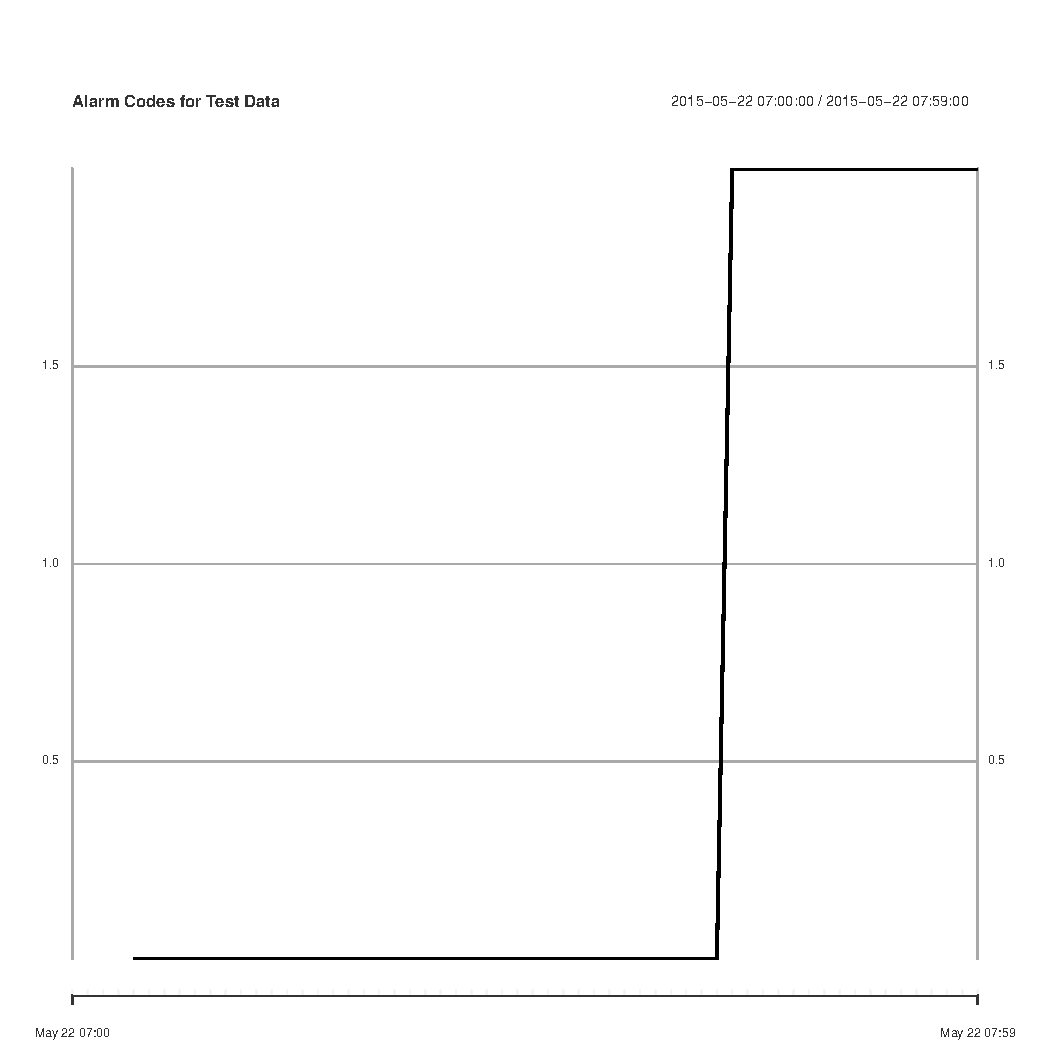
\includegraphics[width=\maxwidth]{figure/r_warning_Plot-1} 

\end{knitrout}
The alarm codes are
\begin{enumerate}
\item ``0'': No alarm.
\item ``1'': Hotelling's $T^2$ alarm.
\item ``2'': Squared Prediction Error alarm.
\item ``3'': Both alarms.
\end{enumerate}
As we can see, the monitoring function detects a process anomaly after 40 minutes into the test hour, and the warning function issues the corresponding alarms.



%%%%%%%%%%%%%%%%%%%%%%%%%%%%%%%%%%%%%%%%%%%%%%%%%%%%%%%%%%%%%%%%%%%%%%%%%%%%%%%
%%%%%%  Conclusion  %%%%%%%%%%%%%%%%%%%%%%%%%%%%%%%%%%%%%%%%%%%%%%%%%%%%%%%%%%%
%%%%%%%%%%%%%%%%%%%%%%%%%%%%%%%%%%%%%%%%%%%%%%%%%%%%%%%%%%%%%%%%%%%%%%%%%%%%%%%

\section{Conclusion} \label{sec:D_Conclusion}
We have supplied our motivation for this package, and we have discussed implementing a multivariate process monitoring scheme with this package using the example of a decentralized WWT plant in Golden, CO. We believe that this software will provide system engineers with the tools necessary to quickly and accurately detect abnormalities in multivariate, autocorrelated, non-stationary, non-linear, and multi-state water treatment systems. Further, we have given a synthetic example showing how the functions within this package would be implemented and tuned in practice.

\end{document}

